% úvod o kapitole, přehled

\section{Strand models}
	
	There exist (can be synthesized) many types of molecules, well described in Winfree \cite{winfree_comp} even with their inception reaction. The most important structures are linear strands (sections \ref{sec:lin_strands}, \ref{sec:adleman}, figure \ref{fig:linear}), dendrimer structures (section \ref{sec:dendrimer}, figure \ref{fig:dendrimer}) and double crossover molecules (section \ref{sec:double_crossover}, figure \ref{fig:double_crossover}).
	\begin{note}\label{note:untwist}
		DNA naturally forms double-helices which would be confusing in figures so there will mostly appear schemes of ``untwisted'' molecules, only double crossover molecules will be described more precisely. % nebo snad unscrewed?
	\end{note}
	
	\subsection{Linear strands}
	\label{sec:lin_strands}
		
		Linear strands are just a piece of double-helix with two types of ends: either with one strand longer than the other (sticky end) or with both strands connected to each other. The top molecule in figure \ref{fig:linear} is called {\em hairpin}.
		\begin{figure}[H]
		\begin{center}
			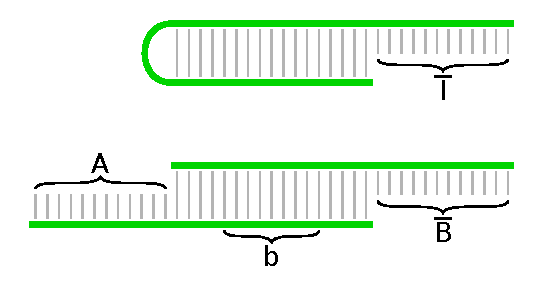
\includegraphics[width=0.502\textwidth]{./figures/strand_types/linear.pdf} % {šířka v mm}/370 je to původně
			\caption{Linear strands: A strand for initial symbol $I$ and a strand for rule $A\rightarrow bB$.}
			\label{fig:linear}
		\end{center}
		\end{figure}
		Winfree \cite{winfree_phd} proved about restricted class of linear strands to be equivalent to regular languages, this means
		\begin{itemize}
			\item given a set of linear strands, the generated language is regular,
			\item given a regular language there exists a set of linear strands which generate it.
		\end{itemize}
		Figure \ref{fig:linear} shows how to assign grammar rules with molecules.
	
	\subsection{Adleman's experiment}
	\label{sec:adleman}
		
		Linear strands were used in Adleman's ground-breaking work \cite{adleman94}. He showed that that DNA molecules are really capable of computation. He exploited that huge parallelism possible in DNA computation for one of the most fundamental $\NP$-complete problems -- the Hamiltonian Path Problem (HPP) in directed graph with designated vertices $v_{begin}$ and $v_{end}$.
		
		Let us remind this type of HPP. Given a directed graph $G_n$ with $n$ vertices and two designated vertices $v_{begin}$ and $v_{end}$, the problem is to answer whether there exists an oriented path from $v_{begin}$ to $v_{end}$ through the graph such that the path visits every vertex. Note that {\em path} cannot visit any vertex more than once from definition.
		
		\begin{figure}[H]
		\begin{center}
			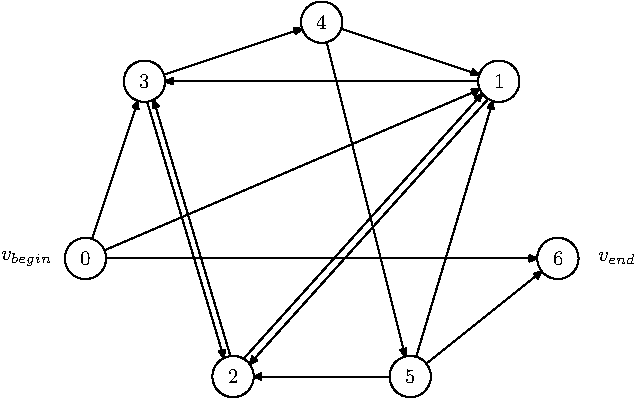
\includegraphics{./figures/adleman_graph.pdf}
			\caption{Adleman's original graph.}
			\label{fig:adleman_graph}
		\end{center}
		\end{figure}
		
		Adleman originally used a graph with seven vertices shown in figure \ref{fig:adleman_graph}. It can be seen that the path $0 \rightarrow 1 \rightarrow 2 \rightarrow 3 \rightarrow 4 \rightarrow 5 \rightarrow 6$ is Hamiltonian\footnote{Note that it can be re-labelled such a nice way without loss of generality.}.
		
		Adleman first presents this non-deterministic five-step algorithm, whose steps are then described in terms of DNA manipulations:
		\begin{description}
			\item[Step 1] Generate random paths through the graph.
			\item[Step 2] Keep only those paths that begin with $v_{begin}$ and end with $v_{end}$.
			\item[Step 3] If the graph has $n$ vertices, then keep only those paths that enter exactly $n$ vertices.
			\item[Step 4] Keep only those paths that enter all of the vertices of the graph at least once.
			\item[Step 5] If any paths remain, say ``Yes''; otherwise, say ``No.''\footnote{This is the original version, I would rectify the fifth step: If any paths remain, say ``Yes''; otherwise say ``{\em I do not know}''. That is because it may happen that there exists a valid path but unfortunately it did not assemble or got lost. Note the similarity to $\NP$ versus $\coNP$, see section \ref{sec:PNP}.} %!% citaci, někdo to už taky kritizoval
		\end{description}
		To see % sloveso od insight ?
		how DNA can compute, let us describe this example more precisely. The computation itself (meaning the inception of the final solution) is hidden in Step 1. Each vertex $i$ is associated with a random\footnote{We will expect those sequences to be different enough.} $20$-mer sequence of DNA, let us denote its $5'\rightarrow 3'$ orientation by $O_i$, its 10-mer prefix by $p_i$ and its 10-mer suffix by $q_i$. Each edge $i\rightarrow j$ is then associated with $\overline{q_i p_j}$ sequence with reverse backbone orientation ($3'\rightarrow 5'$) where $\overline{q_i}$ stands for Watson-Crick complementary word. There is an exception for $i=begin$ and $j=end$: instead of $\overline{q_{begin} p_j}$ there is $\overline{O_{begin} p_j}$ and in a similar way for $j=end$.
		
		\begin{figure}[H]
		\begin{center}
			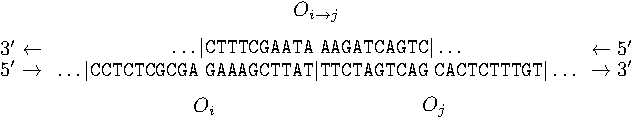
\includegraphics{./figures/adleman_strands.pdf}
			\caption{Example of assigned sequences.}
			\label{fig:adleman_strands}
		\end{center}
		\end{figure}
		
		It can be easily seen that all correctly bonded double-strands correspond with a valid walk through $G_n$. Moreover, all complete double-strands represent a valid walk from $v_{begin}$ to $v_{end}$ through $G_n$.
		
		All the other steps are fully described in \cite{adleman94}. The most important thing is that the most time-demanding step is Step 4. In this step one has to purify the product of Step 3 with a {\em biotin-avidin magnetic beads system}. This process extracts consequently for every vertex $i$ only those DNA strands which contain a substring representing vertex $i$. Thus this algorithm has biostep complexity $O(n)$ which we considered unfeasible. Better solution with biostep complexity $O(1)$ was introduced by Winfree \cite{winfree_phd}, see section \ref{sec:double_crossover}. %!% strašně lžu, tam to třeba vůbec nebude
	
	\subsection{Dendrimer structures}
	\label{sec:dendrimer}
		
		Dendrimer structures are multi-strand molecules which form such trees, see figure \ref{fig:dendrimer}. There can be arbitrary\footnote{In this moment the model is theoretical though practically it has limitations. Note that even with limited number of leafs the size of the whole system must be limited: having $O(2^n)$ molecules, they must fit in space $O(n^3)$ thus $n$ must be limited.} number of leafs and every leaf can be ended by both two ways, see section \ref{sec:lin_strands}. Winfree \cite{winfree_phd} proved similar property as for linear strands: dendrimer structures are equivalent to context-free languages. Figure \ref{fig:dendrimer} shows an example context-free rule.
		
		\begin{figure}[H]
		\begin{center}
			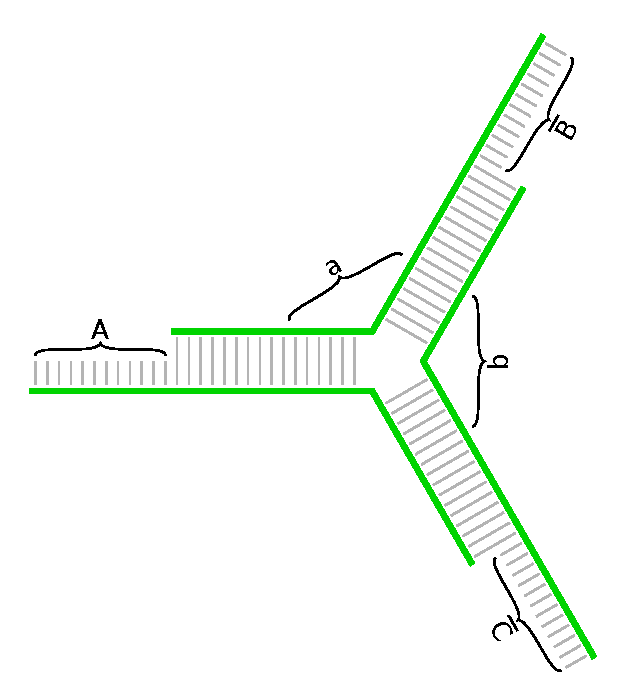
\includegraphics[width=0.568\textwidth]{./figures/strand_types/dendrimer.pdf}
			\caption{Dendrimer structure for rule $A\rightarrow aBbC$.}
			\label{fig:dendrimer}
		\end{center}
		\end{figure}
	
	\subsection{Double crossover molecules}
	\label{sec:double_crossover}
		
		Double crossover molecules are the most important ones. Though they are more complicated they are still very rigid \cite{seeman93}. Moreover they are theoretically capable of universal computation because they can form 2D tilings\footnote{See figure \ref{fig:DNA_assembly} and note how this type of molecules form tilings.} and thus they can simulate cellular automaton \cite{winfree_phd}. As we mentioned in note \ref{note:untwist} we will also describe their inner structure. % universal computation: Winfree pg 57
		
		\begin{figure}[H]
		\begin{center}
			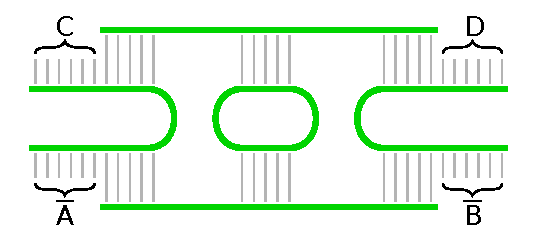
\includegraphics[width=0.492\textwidth]{./figures/strand_types/double_crossover.pdf}
			\caption{Double crossover molecule scheme.}
			\label{fig:double_crossover}
		\end{center}
		\end{figure}
		
		There are many possibilities how those strands can be twisted and connected. The most common ones are DAE and DAO molecules (Double-crossover, Antiparallel helical strands, Even or Odd, respectively, number of half-turns between crossovers), see figure \ref{fig:dao-dae}. It can be seen that DAO molecules form tilings with strands jumping from one stage to another, on the other hand DAE molecules form tilings with a strand leading through entire stage in a row.
		
		Later we will need to read the bottom line's sequence thus it is practically reasonable to use DAE molecules. Moreover we will require even number of half-turns between crossovers in adjacent molecules. This is well explained in \cite[pg. 37]{winfree_phd} on a large figure.
		
		\begin{figure}[H]
		\begin{center}
			\begin{subfigure}[b]{0.433\textwidth} % 130mm/300
				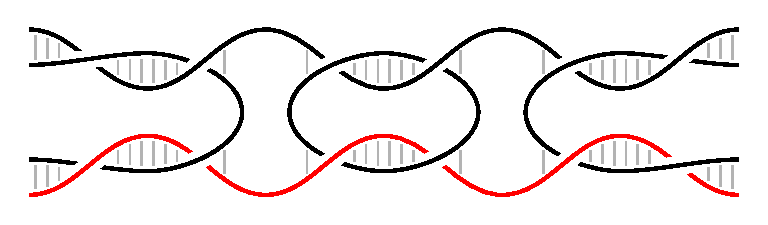
\includegraphics[width=\textwidth]{./figures/dao-dae/dae.pdf}
				\caption{DAE.}
				\label{fig:dao}
			\end{subfigure}
			\begin{subfigure}[b]{0.5\textwidth} % 150mm/300
				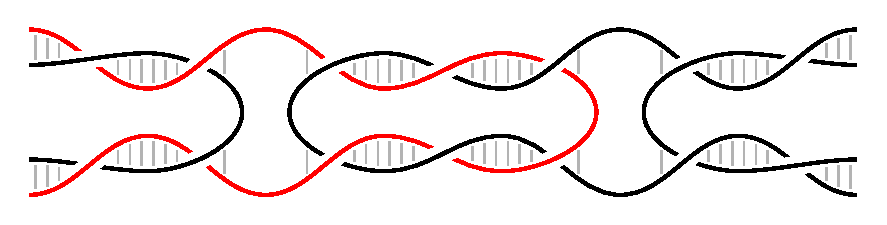
\includegraphics[width=\textwidth]{./figures/dao-dae/dao.pdf}
				\caption{DAO.}
				\label{fig:dae}
			\end{subfigure}
			\caption{DAO vs. DAE.}
			\label{fig:dao-dae}
		\end{center}
		\end{figure}
		
		
		
		DAE molecules seem to be the most promising % citovat tunu praktickejch článků
		thus chapter \ref{chap:problems} will be dedicated spacially to these molecules.
		
		% Biostep complexity $O(1)$ in particular cases.
		
		% Winfree pg 36 -- sizes of DAE and a better picture, pg 37 -- comparison of DAO/DAE in a lattice, explanation pg 43.
		
		% Seeman, Fu \cite{seeman93}, is the picture of DAO strange?
		
		% Important notes in 3.2.5 Winfree -- single side hybridization -- how to avoid.